\label{subsec:network}
The \textit{Lightyear 0's} in-vehicle network is based on a decentralized functional architecture, with CAN and LIN as the main network technologies. Ethernet is used for non-real time applications such as infotainment, over-the-air updates and debugging. This means that networked components pertaining to the same function or domain (body control, drivetrain etc.) are grouped together in a network. The networks are linked together through a \textit{Central Gateway} which bridges the relevant data between networks. For example the \textit{motor power} might be required in the \textit{battery management system}, \textit{propulsion controller} and \textit{media controller}. But for various reasons these controllers might not all be connected to the same network, so the \textit{motor power} needs to be forwarded on the relevant networks.

At the core of the embedded system are three ECUs named the \textit{Central Gateway (CGW)}, \textit{Safety Control Unit (SCU)}, \textit{Vehicle Control Unit (VCU)}. The \textit{Safety Control Unit} is an off the shelf \textit{OpenECU M560} which contains two heterogeneous cores, that both have access to the connected CAN busses. The \textit{Vehicle Control Unit} is also an \textit{OpenECU M560}, but the secondary core is not used, while the \textit{Central Gateway} uses a \textit{OpenECU M130}. Each ECU has a real-time operating system with a fixed priority preemptive scheduler and can be connected up to four CAN busses and two LIN busses. While the RTOS is provided by the manufacturer of the \textit{OpenECUs} the software running inside the RTOS is developed by Lightyear and thus the functionality of an ECU is not fixed. For this reason we will call these ECUs \textit{programmable end nodes} for modelling purposes.

The other nodes in the network have a fixed function, some of them are developed by Lightyear such as motor inverters and solar converters, while others are developed by third parties. Some of these can be configured by the user to tune the behaviour, while others are completely fixed. For modelling purposes we call these nodes \textit{parametrizable end nodes}. The inner workings of these nodes varies and is unknown in case of a third party component. Fortunately for network simulation only the external behaviour needs to be known. Because these nodes must be integrated, a precise specification of the network traffic generated and consumed should be available and thus can be used when modelling a node.

From Lightyear's internal documentation we were able to generate an overview of all the networks in the car and which nodes connect to which network. The two LIN busses, LIN A and LIN B, each connect to the \textit{Central Gateway} which acts as the master in the LIN networks. The slave nodes are third party of the shelf components and can be classified as \textit{parametrizable end nodes}. Table~\ref{tab:networkoverview} represents a partial overview of the nodes, the networks and their connections in the Lightyear 0. Unfortunately Lightyear's documentation was not complete and retrieving the relevant information of every node would have taken a significant effort. Due to time reasons a subset of the nodes mentioned in the table have been modelled, those have been coloured green. An alternative schematic overview can be found in Figure~\ref{fig:networkoverview}.

Finally, there are components in the vehicle that generate or consume data but are not seen as a networked component in the "traditional" sense. Examples are speakers, rearview cameras and instrument cluster displays. Further investigation is necessary to determine how many of these nodes exist, how they are connected and how they should be modelled from a networking perspective.
\begingroup
\renewcommand*{\arraystretch}{1}
\begin{table}[htb]
    \centering
    \resizebox{\textwidth}{!}{%
    % \begin{tabular}{@{}lllllllllllllllllll@{}}
    \begin{tabular}{lllllllllllllllllll}
                                & \multicolumn{10}{c}{Controller Area Network} & \multicolumn{2}{c|}{LIN} & \multicolumn{5}{c}{Ethernet} & \multicolumn{1}{c}{Other} \\* \cmidrule(lr){2-11} \cmidrule(r){12-13} \cmidrule(r){14-18} \cmidrule(r){19-19}
    Node name                & \multicolumn{1}{R{2.5cm}}{Driver support} & \multicolumn{1}{R{2cm}}{Drivetrain} & \multicolumn{1}{R{2cm}}{Energy\\ management} & \multicolumn{1}{R{2cm}}{HVBS} & \multicolumn{1}{R{2cm}}{Powertrain} & \multicolumn{1}{R{2cm}}{Solar} & \multicolumn{1}{R{2cm}}{Surrounding\\ sense} & \multicolumn{1}{R{2cm}}{Telematics} & \multicolumn{1}{R{2cm}}{Vehicle} & \multicolumn{1}{R{2cm}}{Vehicle 2} & \multicolumn{1}{R{2cm}}{LIN A} & \multicolumn{1}{R{2cm}|}{LIN B} & \multicolumn{1}{R{2cm}}{Media} & \multicolumn{1}{R{2cm}}{Inverter FL} & \multicolumn{1}{R{2cm}}{Inverter FR} & \multicolumn{1}{R{2cm}}{Inverter RL} & \multicolumn{1}{R{2cm}}{Inverter RR} & \multicolumn{1}{R{2cm}}{Others}   \\*\cmidrule(r){1-1} \cmidrule(r){2-11}\cmidrule(r){12-13} \cmidrule(r){14-18} \cmidrule(r){19-19}
    \textcolor{mint}{Vehicle control unit}       & X &   &   &   &   & X & X &   & X &   &   & \multicolumn{1}{c|}{}  &   &   &   &   &   &   \\
    \rowcolor[gray]{0.925}
    \textcolor{mint}{Central gateway}            &   &   &   &   & X &   &   & X & X & X & X & \multicolumn{1}{c|}{X} &   &   &   &   &   &   \\
    \textcolor{mint}{Safety control unit}        &   & X & X & X & X &   &   &   &   &   &   & \multicolumn{1}{c|}{}  &   &   &   &   &   &   \\
    \rowcolor[gray]{0.925}
    \textcolor{mint}{Steering column module}     & X &   &   &   &   &   &   &   &   &   &   & \multicolumn{1}{c|}{}  &   &   &   &   &   &   \\
    \textcolor{mint}{Inverter FL}                &   & X &   &   &   &   &   &   &   &   &   & \multicolumn{1}{c|}{}  &   & X &   &   &   &   \\
    \rowcolor[gray]{0.925}
    \textcolor{mint}{Inverter FR}                &   & X &   &   &   &   &   &   &   &   &   & \multicolumn{1}{c|}{}  &   &   & X &   &   &   \\
    \textcolor{mint}{Inverter RL}                &   & X &   &   &   &   &   &   &   &   &   & \multicolumn{1}{c|}{}  &   &   &   & X &   &   \\
    \rowcolor[gray]{0.925}
    \textcolor{mint}{Inverter RR}                &   & X &   &   &   &   &   &   &   &   &   & \multicolumn{1}{c|}{}  &   &   &   &   & X &   \\
    High voltage battery                         &   &   &   & X &   &   &   &   &   &   &   & \multicolumn{1}{c|}{}  &   &   &   &   &   &   \\
    \rowcolor[gray]{0.925}
    On-board charger                             &   &   & X &   &   &   &   &   &   &   &   & \multicolumn{1}{c|}{}  &   &   &   &   &   &   \\
    \textcolor{mint}{Media ECU}                  &   &   &   &   & X &   &   &   &   &   &   & \multicolumn{1}{c|}{}  & X &   &   &   &   & X \\
    \rowcolor[gray]{0.925}
    Steering angle sensor                        &   &   &   &   & X &   &   &   &   &   &   & \multicolumn{1}{c|}{}  &   &   &   &   &   &   \\
    \textcolor{mint}{Dual string controller 1}   &   &   &   &   &   & X &   &   &   &   &   & \multicolumn{1}{c|}{}  &   &   &   &   &   &   \\
    \rowcolor[gray]{0.925}
    \textcolor{mint}{Dual string controller 2}   &   &   &   &   &   & X &   &   &   &   &   & \multicolumn{1}{c|}{}  &   &   &   &   &   &   \\
    \textcolor{mint}{Dual string controller 3}   &   &   &   &   &   & X &   &   &   &   &   & \multicolumn{1}{c|}{}  &   &   &   &   &   &   \\
    \rowcolor[gray]{0.925}
    \textcolor{mint}{Dual string controller 4}   &   &   &   &   &   & X &   &   &   &   &   & \multicolumn{1}{c|}{}  &   &   &   &   &   &   \\
    \textcolor{mint}{Dual string controller 5}   &   &   &   &   &   & X &   &   &   &   &   & \multicolumn{1}{c|}{}  &   &   &   &   &   &   \\
    \rowcolor[gray]{0.925}
    \textcolor{mint}{Dual string controller 6}   &   &   &   &   &   & X &   &   &   &   &   & \multicolumn{1}{c|}{}  &   &   &   &   &   &   \\
    \textcolor{mint}{Dual string controller 7}   &   &   &   &   &   & X &   &   &   &   &   & \multicolumn{1}{c|}{}  &   &   &   &   &   &   \\
    \rowcolor[gray]{0.925}
    \textcolor{mint}{Dual string controller 8}   &   &   &   &   &   & X &   &   &   &   &   & \multicolumn{1}{c|}{}  &   &   &   &   &   &   \\
    \textcolor{mint}{Dual string controller 9}   &   &   &   &   &   & X &   &   &   &   &   & \multicolumn{1}{c|}{}  &   &   &   &   &   &   \\
    \rowcolor[gray]{0.925}
    \textcolor{mint}{Dual string controller 10}  &   &   &   &   &   & X &   &   &   &   &   & \multicolumn{1}{c|}{}  &   &   &   &   &   &   \\
    \textcolor{mint}{Dual string controller 11}  &   &   &   &   &   & X &   &   &   &   &   & \multicolumn{1}{c|}{}  &   &   &   &   &   &   \\
    \rowcolor[gray]{0.925}
    \textcolor{mint}{Dual string controller 12}  &   &   &   &   &   & X &   &   &   &   &   & \multicolumn{1}{c|}{}  &   &   &   &   &   &   \\
    \textcolor{mint}{Dual string controller 13}  &   &   &   &   &   & X &   &   &   &   &   & \multicolumn{1}{c|}{}  &   &   &   &   &   &   \\
    \rowcolor[gray]{0.925}
    \textcolor{mint}{Dual string controller 14}  &   &   &   &   &   & X &   &   &   &   &   & \multicolumn{1}{c|}{}  &   &   &   &   &   &   \\
    Camera monitoring system                     &   &   &   &   &   &   & X &   &   &   &   & \multicolumn{1}{c|}{}  &   &   &   &   &   &   \\
    \rowcolor[gray]{0.925}
    \textcolor{mint}{Parking sensor 1}           &   &   &   &   &   &   & X &   &   &   &   & \multicolumn{1}{c|}{}  &   &   &   &   &   &   \\
    \textcolor{mint}{Parking sensor 2}           &   &   &   &   &   &   & X &   &   &   &   & \multicolumn{1}{c|}{}  &   &   &   &   &   &   \\
    \rowcolor[gray]{0.925}
    \textcolor{mint}{Parking sensor 3}           &   &   &   &   &   &   & X &   &   &   &   & \multicolumn{1}{c|}{}  &   &   &   &   &   &   \\
    \textcolor{mint}{Parking sensor 4}           &   &   &   &   &   &   & X &   &   &   &   & \multicolumn{1}{c|}{}  &   &   &   &   &   &   \\
    \rowcolor[gray]{0.925}
    \textcolor{mint}{Parking sensor 5}           &   &   &   &   &   &   & X &   &   &   &   & \multicolumn{1}{c|}{}  &   &   &   &   &   &   \\
    \textcolor{mint}{Parking sensor 6}           &   &   &   &   &   &   & X &   &   &   &   & \multicolumn{1}{c|}{}  &   &   &   &   &   &   \\
    \rowcolor[gray]{0.925}
    \textcolor{mint}{Parking sensor 7}           &   &   &   &   &   &   & X &   &   &   &   & \multicolumn{1}{c|}{}  &   &   &   &   &   &   \\
    \textcolor{mint}{Parking sensor 8}           &   &   &   &   &   &   & X &   &   &   &   & \multicolumn{1}{c|}{}  &   &   &   &   &   &   \\
    \rowcolor[gray]{0.925}
    Telematics control unit                      &   &   &   &   &   &   &   & X &   &   &   & \multicolumn{1}{c|}{}  & X &   &   &   &   &   \\
    Window wiper                                 &   &   &   &   &   &   &   &   & X &   &   & \multicolumn{1}{c|}{}  &   &   &   &   &   &   \\
    \rowcolor[gray]{0.925}
    \textcolor{mint}{RC compressor}              &   &   &   &   &   &   &   &   & X &   &   & \multicolumn{1}{c|}{}  &   &   &   &   &   &   \\
    \textcolor{mint}{Tailgate latch}             &   &   &   &   &   &   &   &   &   & X &   & \multicolumn{1}{c|}{}  &   &   &   &   &   &   \\
    \rowcolor[gray]{0.925}
    \textcolor{mint}{User authentication system} &   &   &   &   &   &   &   &   &   & X &   & \multicolumn{1}{c|}{}  &   &   &   &   &   &   \\
    \textcolor{mint}{User authentication app}    &   &   &   &   &   &   &   & X &   &   &   & \multicolumn{1}{c|}{}  &   &   &   &   &   &   \\
    \rowcolor[gray]{0.925}
    \textcolor{mint}{Alarm system}               &   &   &   &   & X &   &   &   &   &   &   & \multicolumn{1}{c|}{}  &   &   &   &   &   &   \\
    \textcolor{mint}{Front left door latch}      &   &   &   &   & X &   &   &   &   &   &   & \multicolumn{1}{c|}{}  &   &   &   &   &   &   \\
    \rowcolor[gray]{0.925}
    \textcolor{mint}{Front right door latch}     &   &   &   &   &   &   &   &   &   & X &   & \multicolumn{1}{c|}{}  &   &   &   &   &   &   \\
    \textcolor{mint}{Rear left door latch}       &   &   &   &   &   &   &   &   &   & X &   & \multicolumn{1}{c|}{}  &   &   &   &   &   &   \\
    \rowcolor[gray]{0.925}
    \textcolor{mint}{Rear right door latch}      &   &   &   &   & X &   &   &   &   &   &   & \multicolumn{1}{c|}{}  &   &   &   &   &   &   \\
    \textcolor{mint}{Filling tool}               &   &   &   &   &   &   &   &   & X &   &   & \multicolumn{1}{c|}{}  &   &   &   &   &   &   \\
    \rowcolor[gray]{0.925}
    Rain light sensor                            &   &   &   &   &   &   &   &   &   &   & X & \multicolumn{1}{c|}{}  &   &   &   &   &   &   \\
    Air flap actuator                            &   &   &   &   &   &   &   &   &   &   &   & \multicolumn{1}{c|}{X} &   &   &   &   &   &   \\
    \rowcolor[gray]{0.925}
    Speaker left                                 &   &   &   &   &   &   &   &   &   &   &   & \multicolumn{1}{c|}{}  &   &   &   &   &   & X \\
    Display                                      &   &   &   &   &   &   &   &   &   &   &   & \multicolumn{1}{c|}{}  &   &   &   &   &   & X \\
    \rowcolor[gray]{0.925}
    Rearview camera                              &   &   &   &   &   &   &   &   &   &   &   & \multicolumn{1}{c|}{}  &   &   &   &   &   & X \\
\end{tabular}%
}
\caption{Partial overview of in-vehicle networks and nodes}
\label{tab:networkoverview}
\end{table}
\endgroup

\begin{figure}[htb]
    \centering
    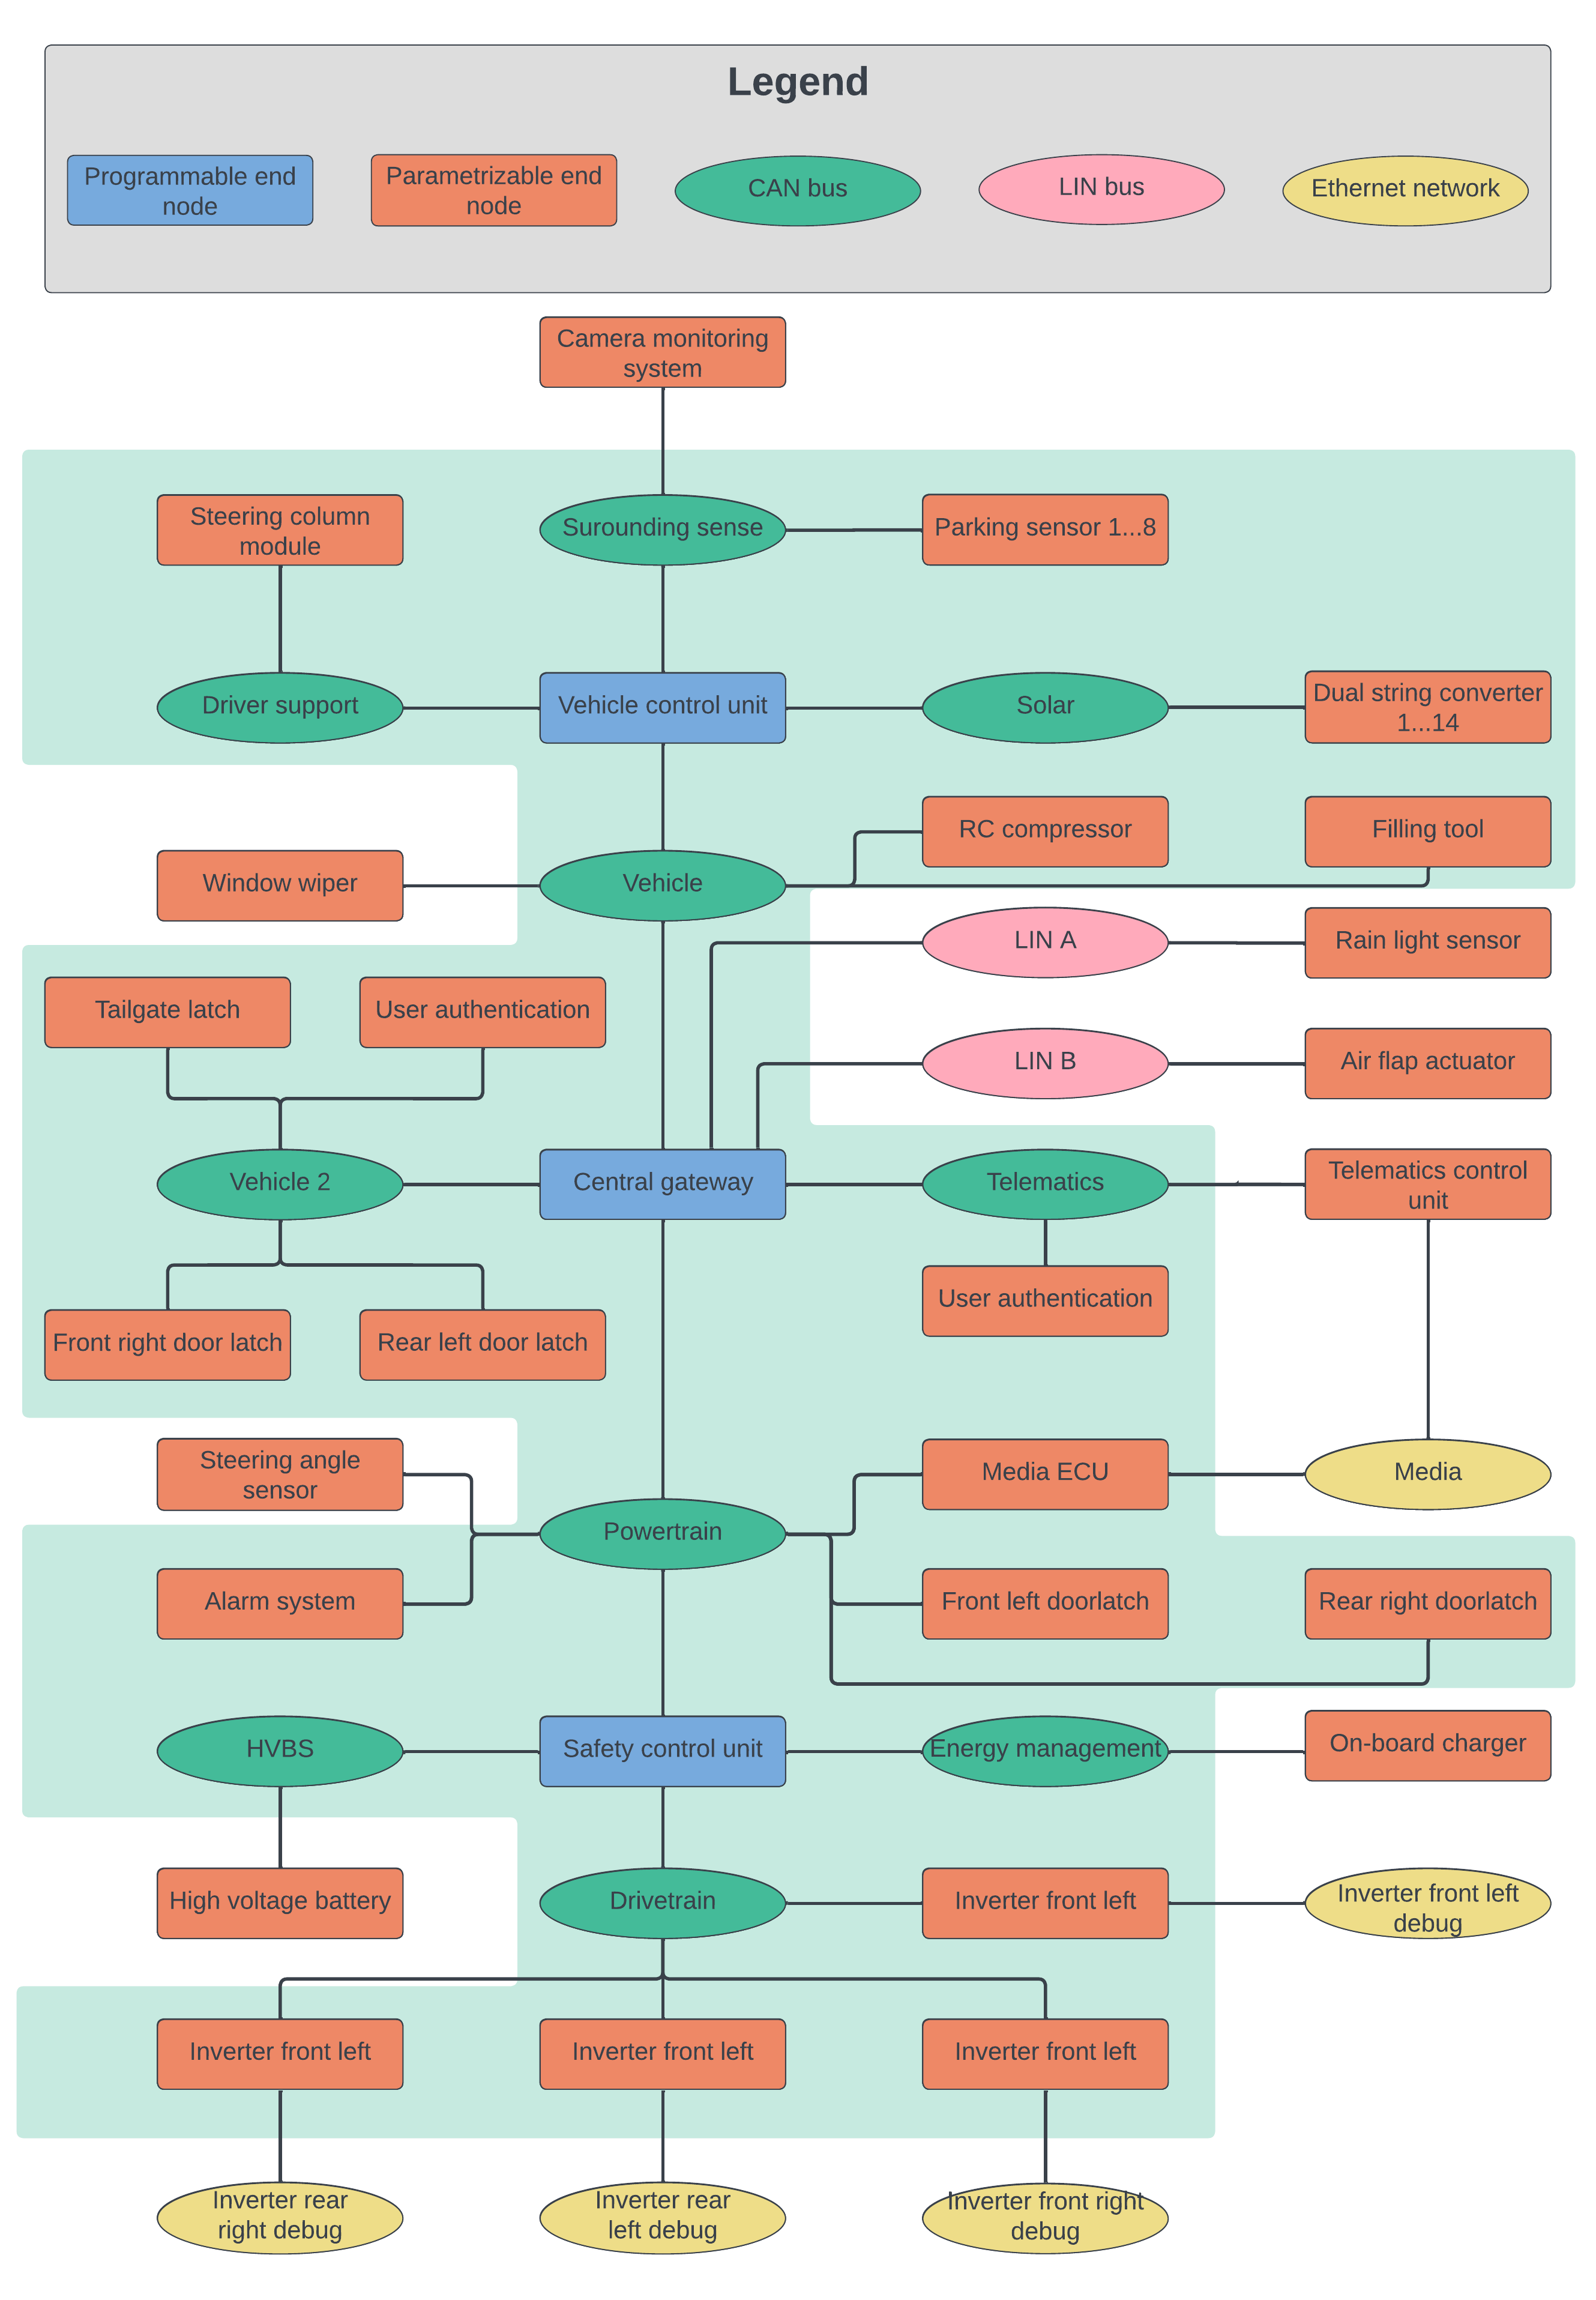
\includegraphics[width=0.95\textwidth]{images/Network_overview.png}
    \caption{Partial overview of the Lightyear 0's in-vehicle network, highlighted in green are the nodes and networks which have been modelled.}
    \label{fig:networkoverview}
\end{figure}
\clearpage